\chapter{Reflectie}
In dit hoofdstuk reflecteer ik op mijn beroepsmatig handelen in het afstudeerproject. Deze reflectie voer ik uit aan de hand van situatiebeschrijvingen die volgens de STARRT methode zijn uitgewerkt. Deze situatiebeschrijvingen zijn opgesteld in het kader van:
\begin{itemize} 
	\item Mijn werkwijze en gemaakte keuzes ten aanzien van de projectuitvoering;
	\item Het toegepaste theoretisch kader;
	\item Het resultaat en de consequenties van het resultaat voor de organisatie.
\end{itemize}
Deze reflectie wordt gestructureerd gedaan op 4 kritische situaties in de volgende situatiebeschrijving zijn volgens de STARRT methode.

\section{Situatiebeschrijvingen}

\subsection{Projectaanpak keuze}
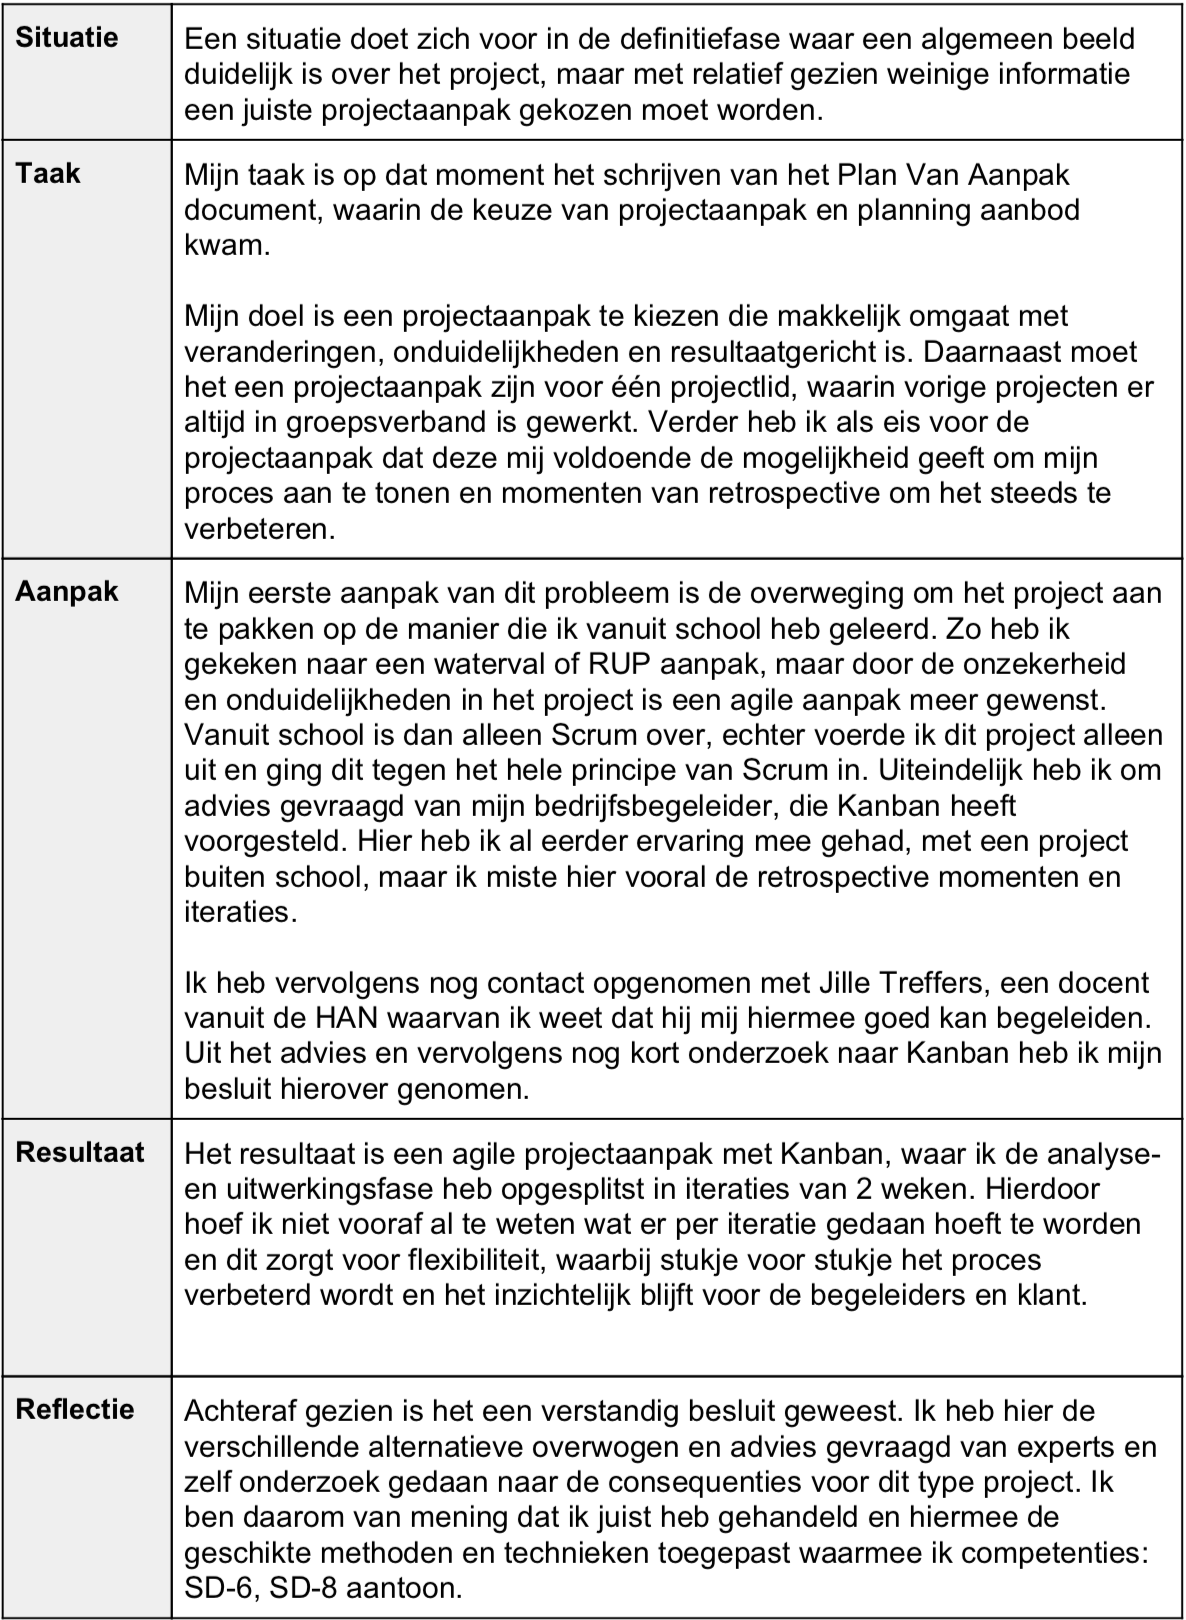
\includegraphics[width=\paperwidth-200]{images/sit_projectaanpak}

\subsection{Communicatie met de opdrachtgever}
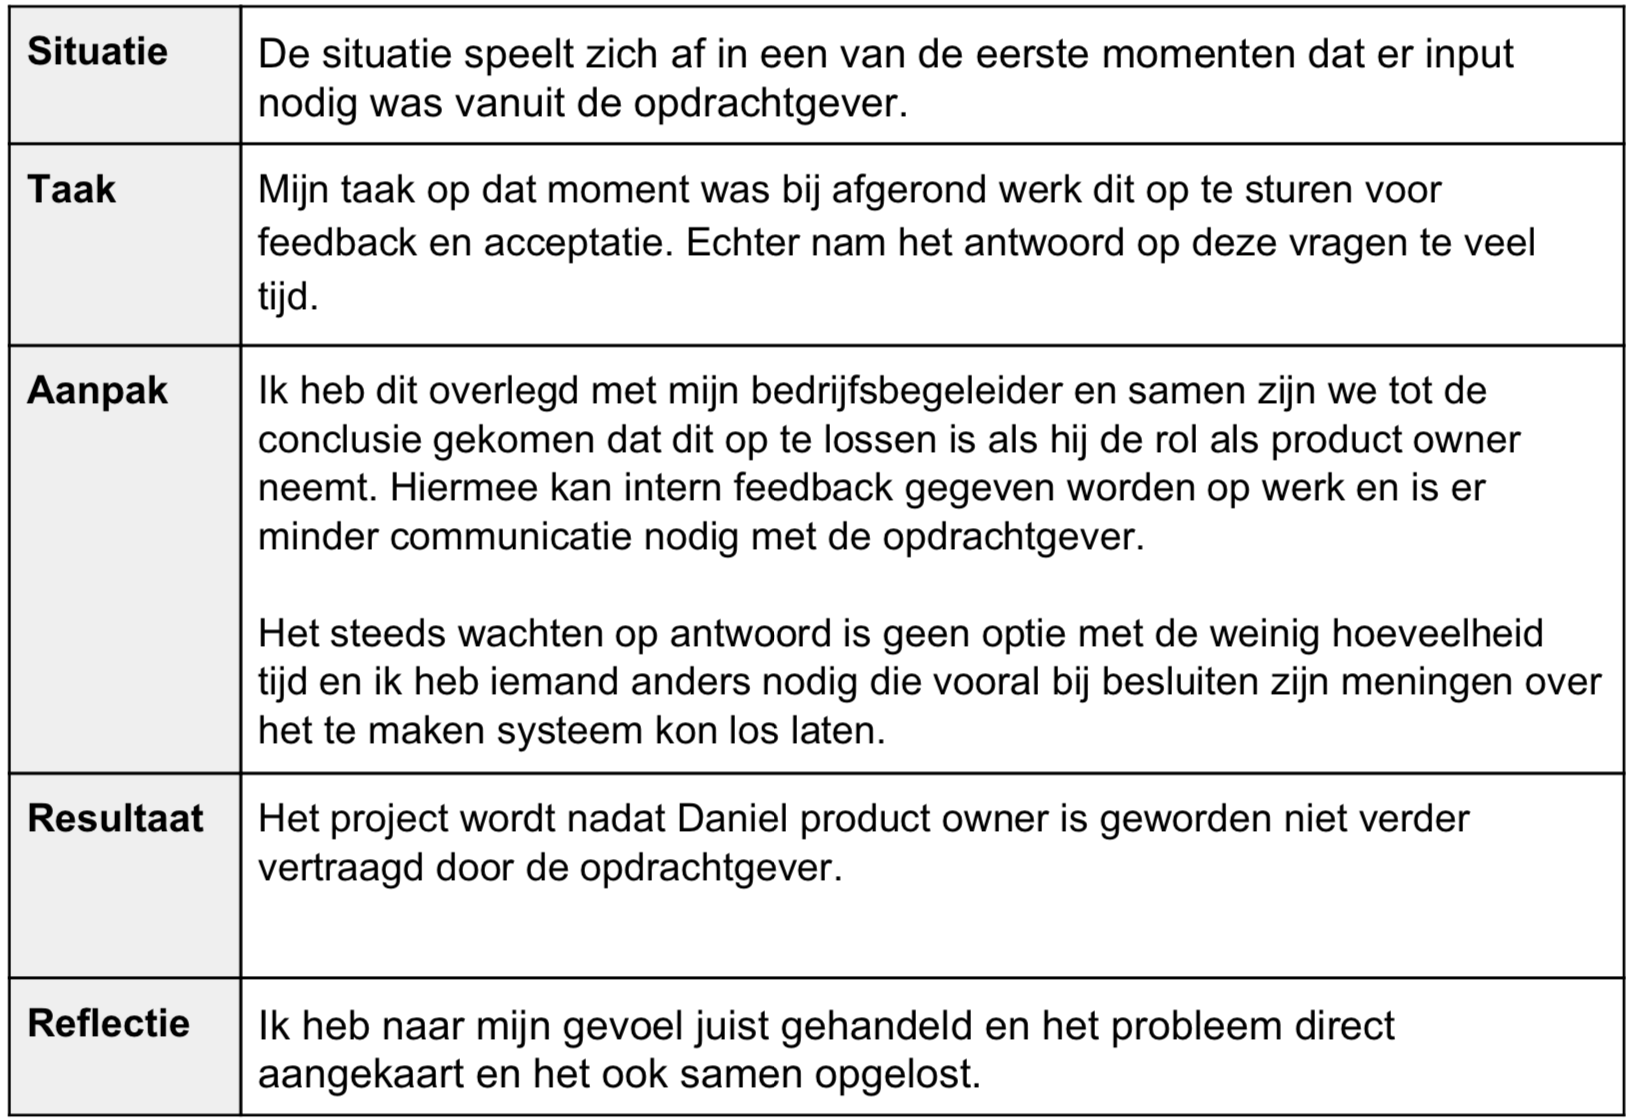
\includegraphics[width=\paperwidth-200]{images/sit_comm}

\subsection{Oplossingsrichtingen planmatig vergelijken}
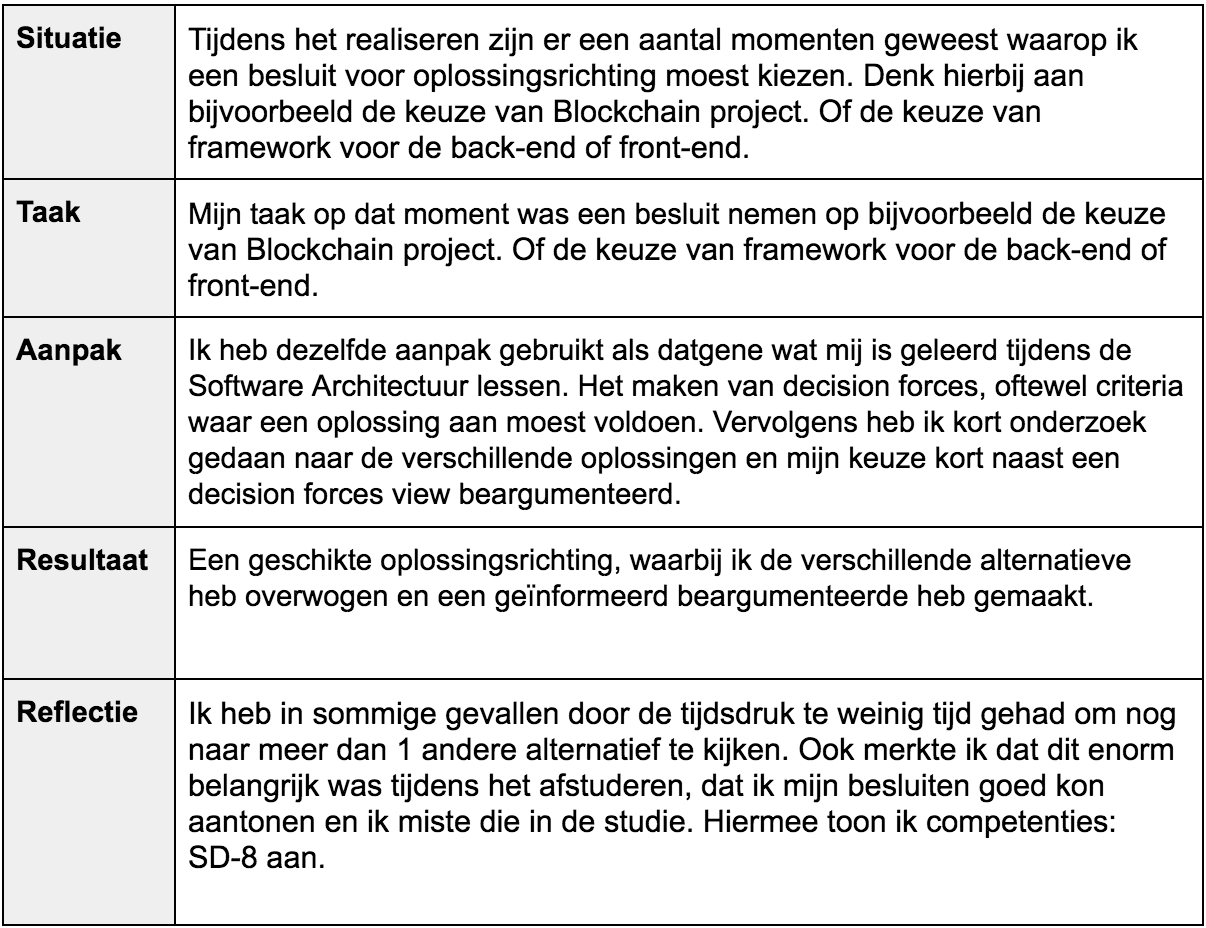
\includegraphics[width=\paperwidth-200]{images/sit_oplossingrichting}

\subsection{Analyse software design documenteren}
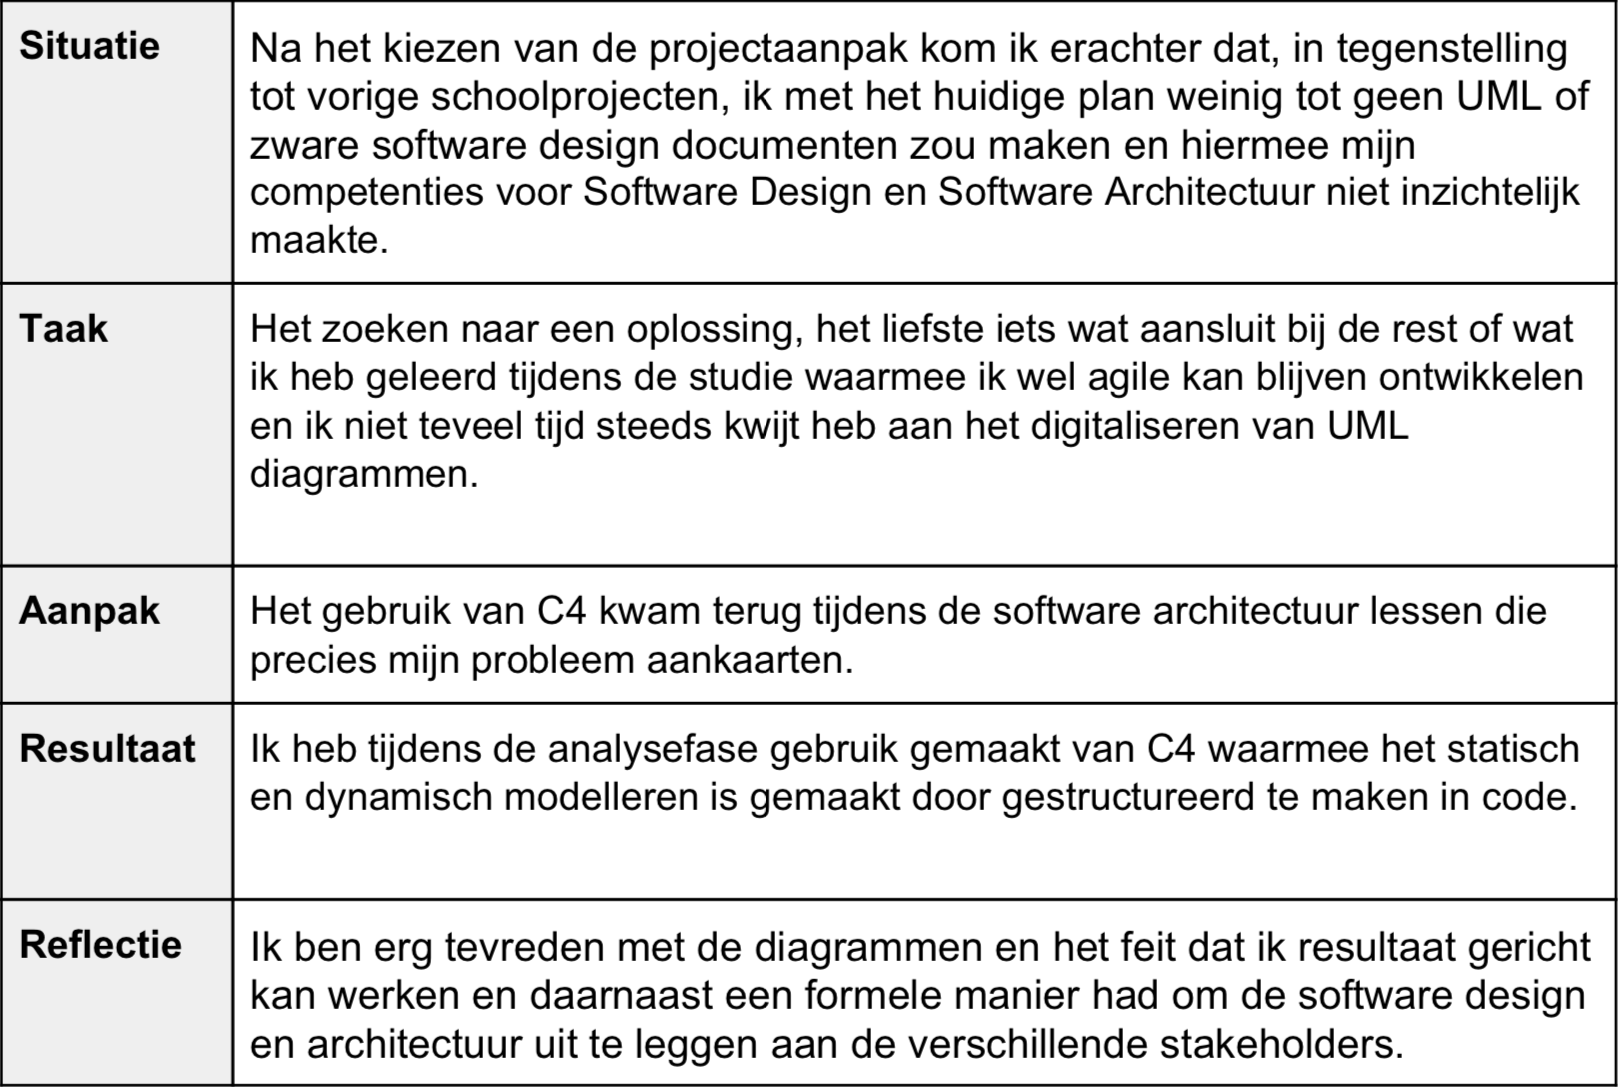
\includegraphics[width=\paperwidth-200]{images/sit_modelana}